\documentclass{standalone}
%
\usepackage{tikz}
\usetikzlibrary{backgrounds,shapes.callouts}
\usepackage{tkz-euclide}
\usepackage{xcolor}
\usepackage{ifthen}
%
\definecolor{space}{HTML}{1F2C4E}
\definecolor{earth}{HTML}{0089FA}
\definecolor{dida}{HTML}{FFDE00}
\definecolor{title}{HTML}{FBA706}
\definecolor{moon}{HTML}{AFAFAF}
%
\usepackage{fontspec}
\setmainfont{Open Dyslexic}
%
\title{Un uccello (forse) tra le stelle}
\begin{document}
	\tikzset{
		partial ellipse/.style args = {#1:#2:#3}{insert path={+ (#1:#3) arc (#1:#2:#3)}},
		notice/.style  = { draw, ellipse callout, callout relative pointer={#1} },
	}
	\begin{tikzpicture}[background rectangle/.style={fill=white},show background rectangle,>={[inset=0,angle'=27]Stealth}]
		%title
		\draw [black,ultra thick] (1,1) rectangle (29,-1);
		\node at (15,0) {\textcolor{black}{\fontsize{40}{41}\selectfont Un uccello (forse) tra le stelle}};
		%
		\begin{scope}[shift={(0,-5)}]
			\node at (3,0) {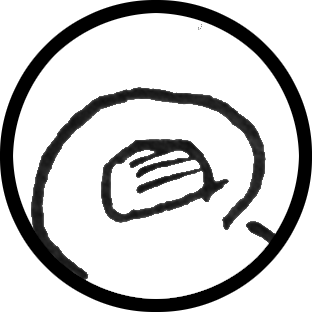
\includegraphics[width=5cm]{img-archaeopteryx/qfwfq_tondino}};
			\node (example-textwidth-2) [right, align=left, text width=22cm, color=black, font=\fontsize{18pt}{19pt}\selectfont] at (6,0) {Mi sono trasferito su questo sasso spaziale nel 1991, dopo che Eric Walter Elst lo scopri' grazie ai suoi strumenti astronomici. Direi che, per le mie spartane esigenze, e' piu' che sufficiente con i suoi 12 km di diametro!};
		\end{scope}
		% 
		\begin{scope}[shift={(0,-14)}]
			\node at (15,0) {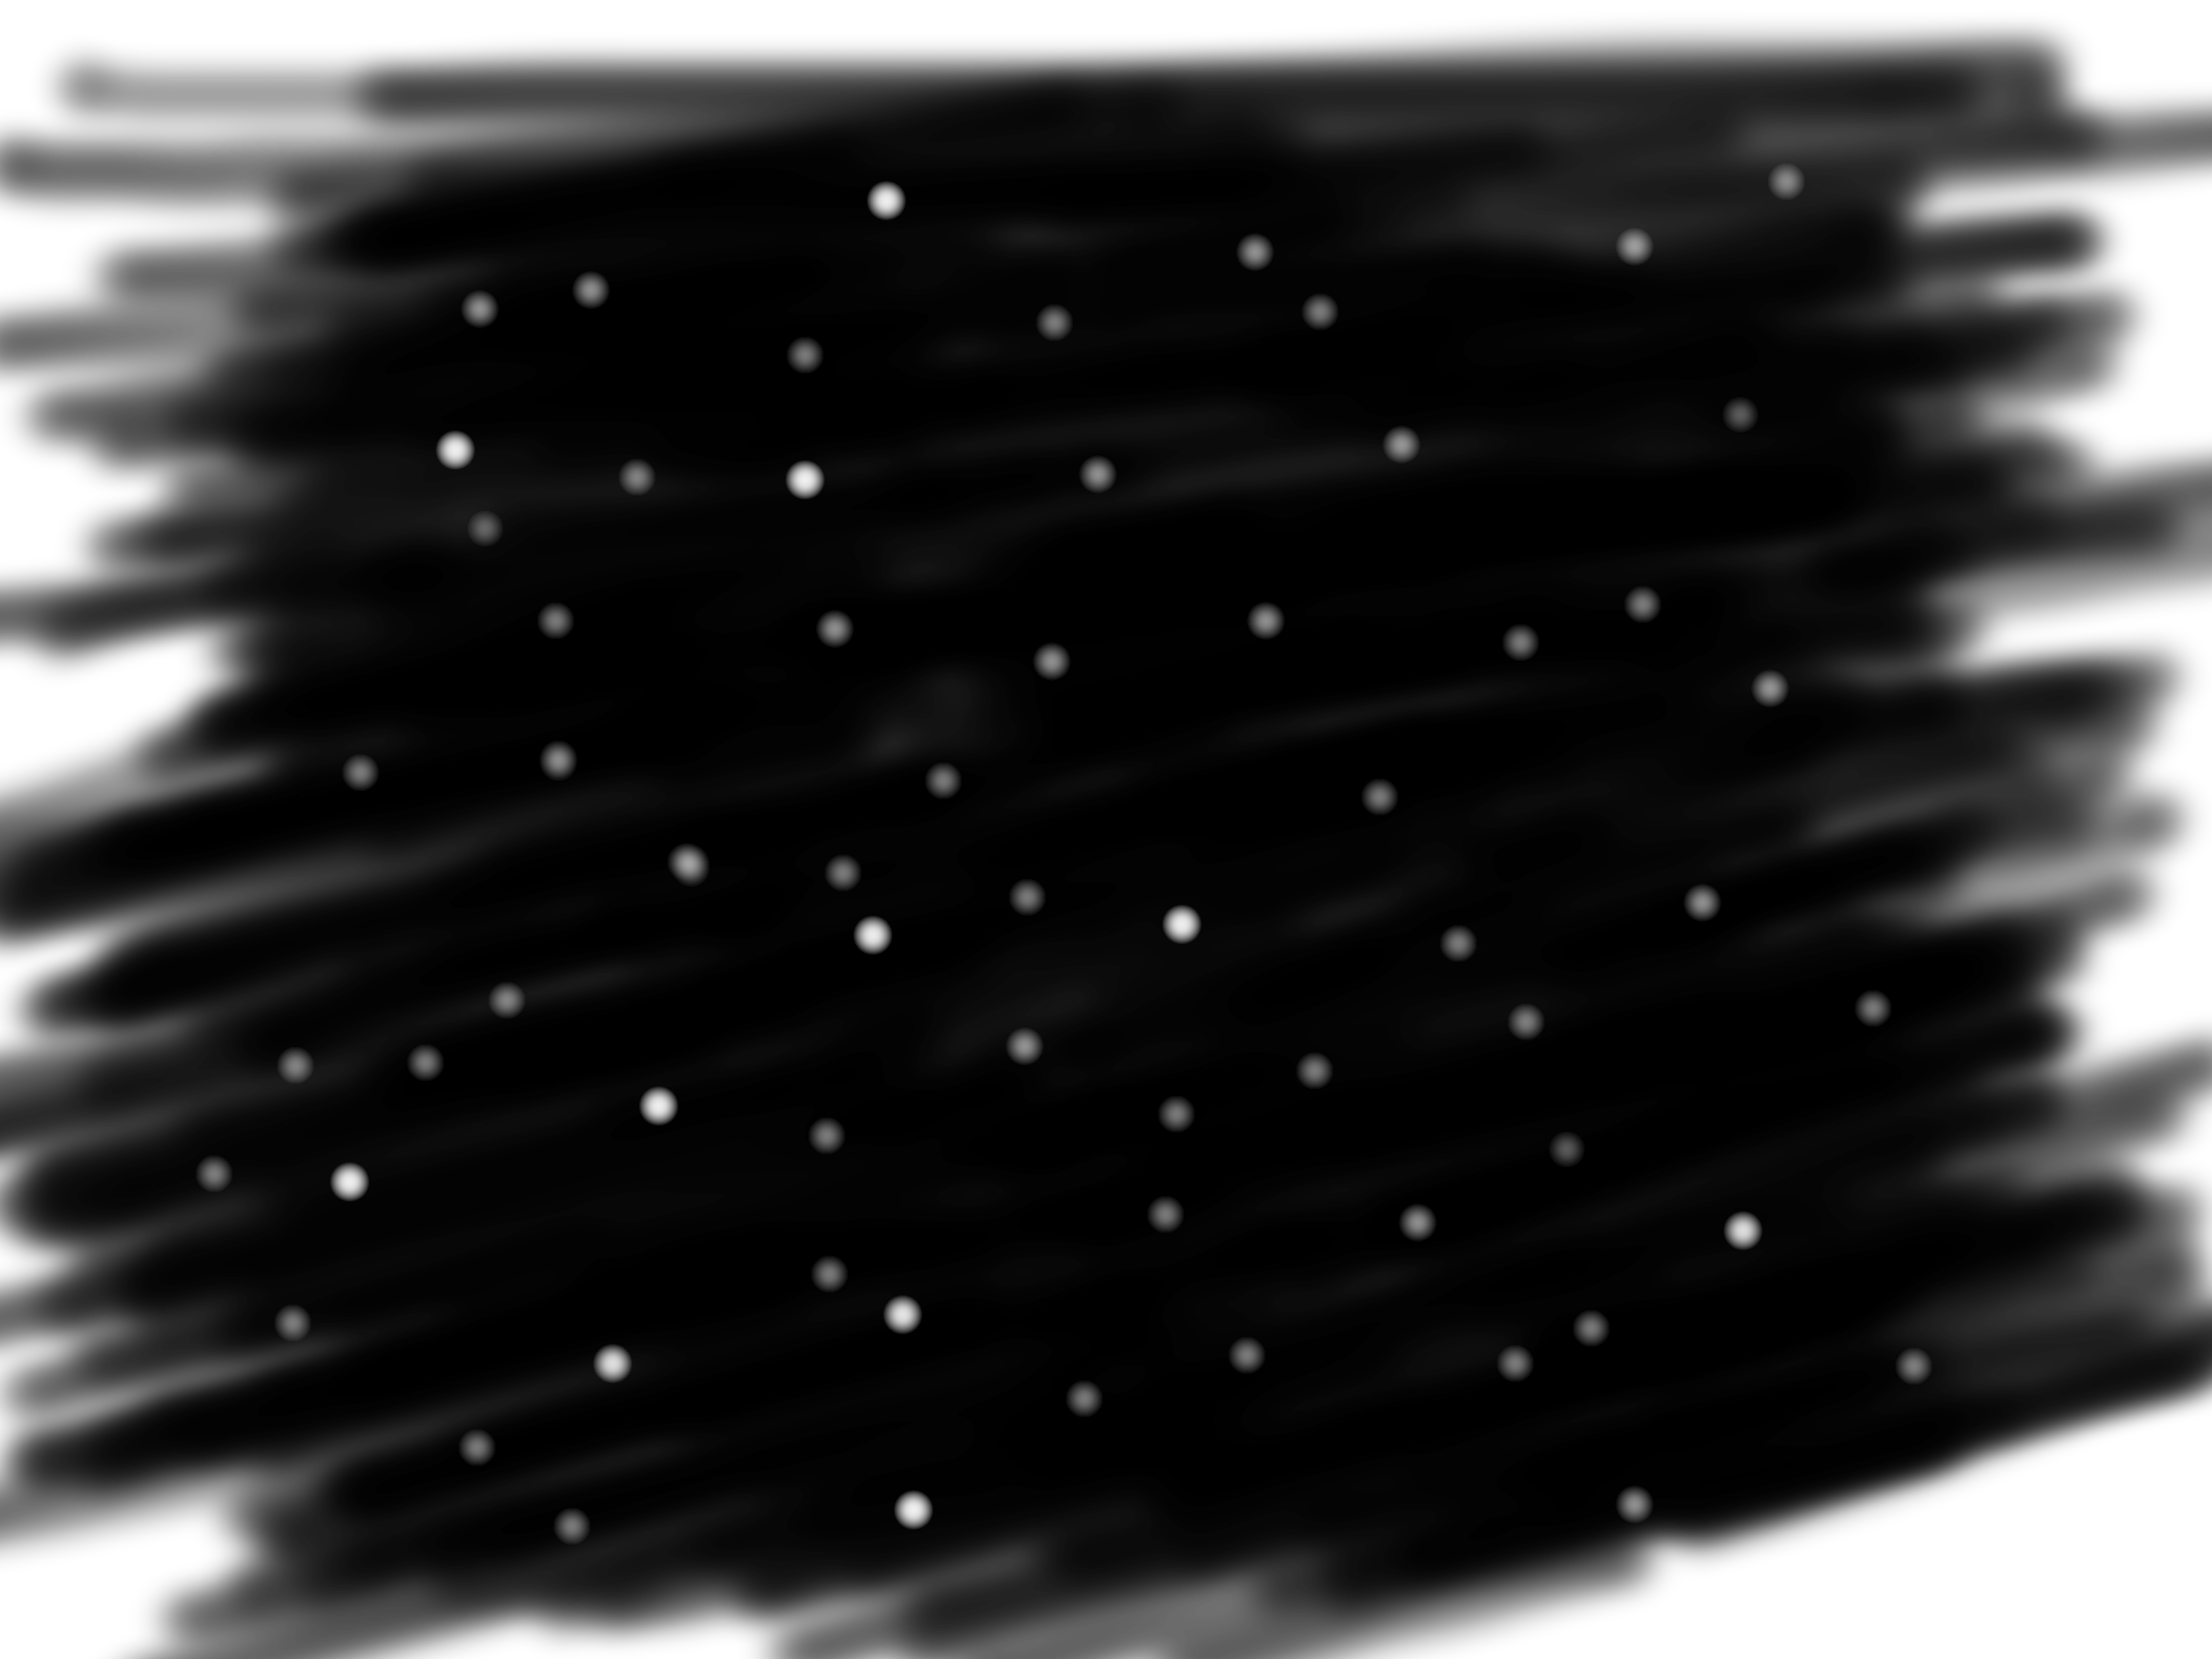
\includegraphics[width=18cm]{img-archaeopteryx/cielo_stellato}};
			\node at (15,0) {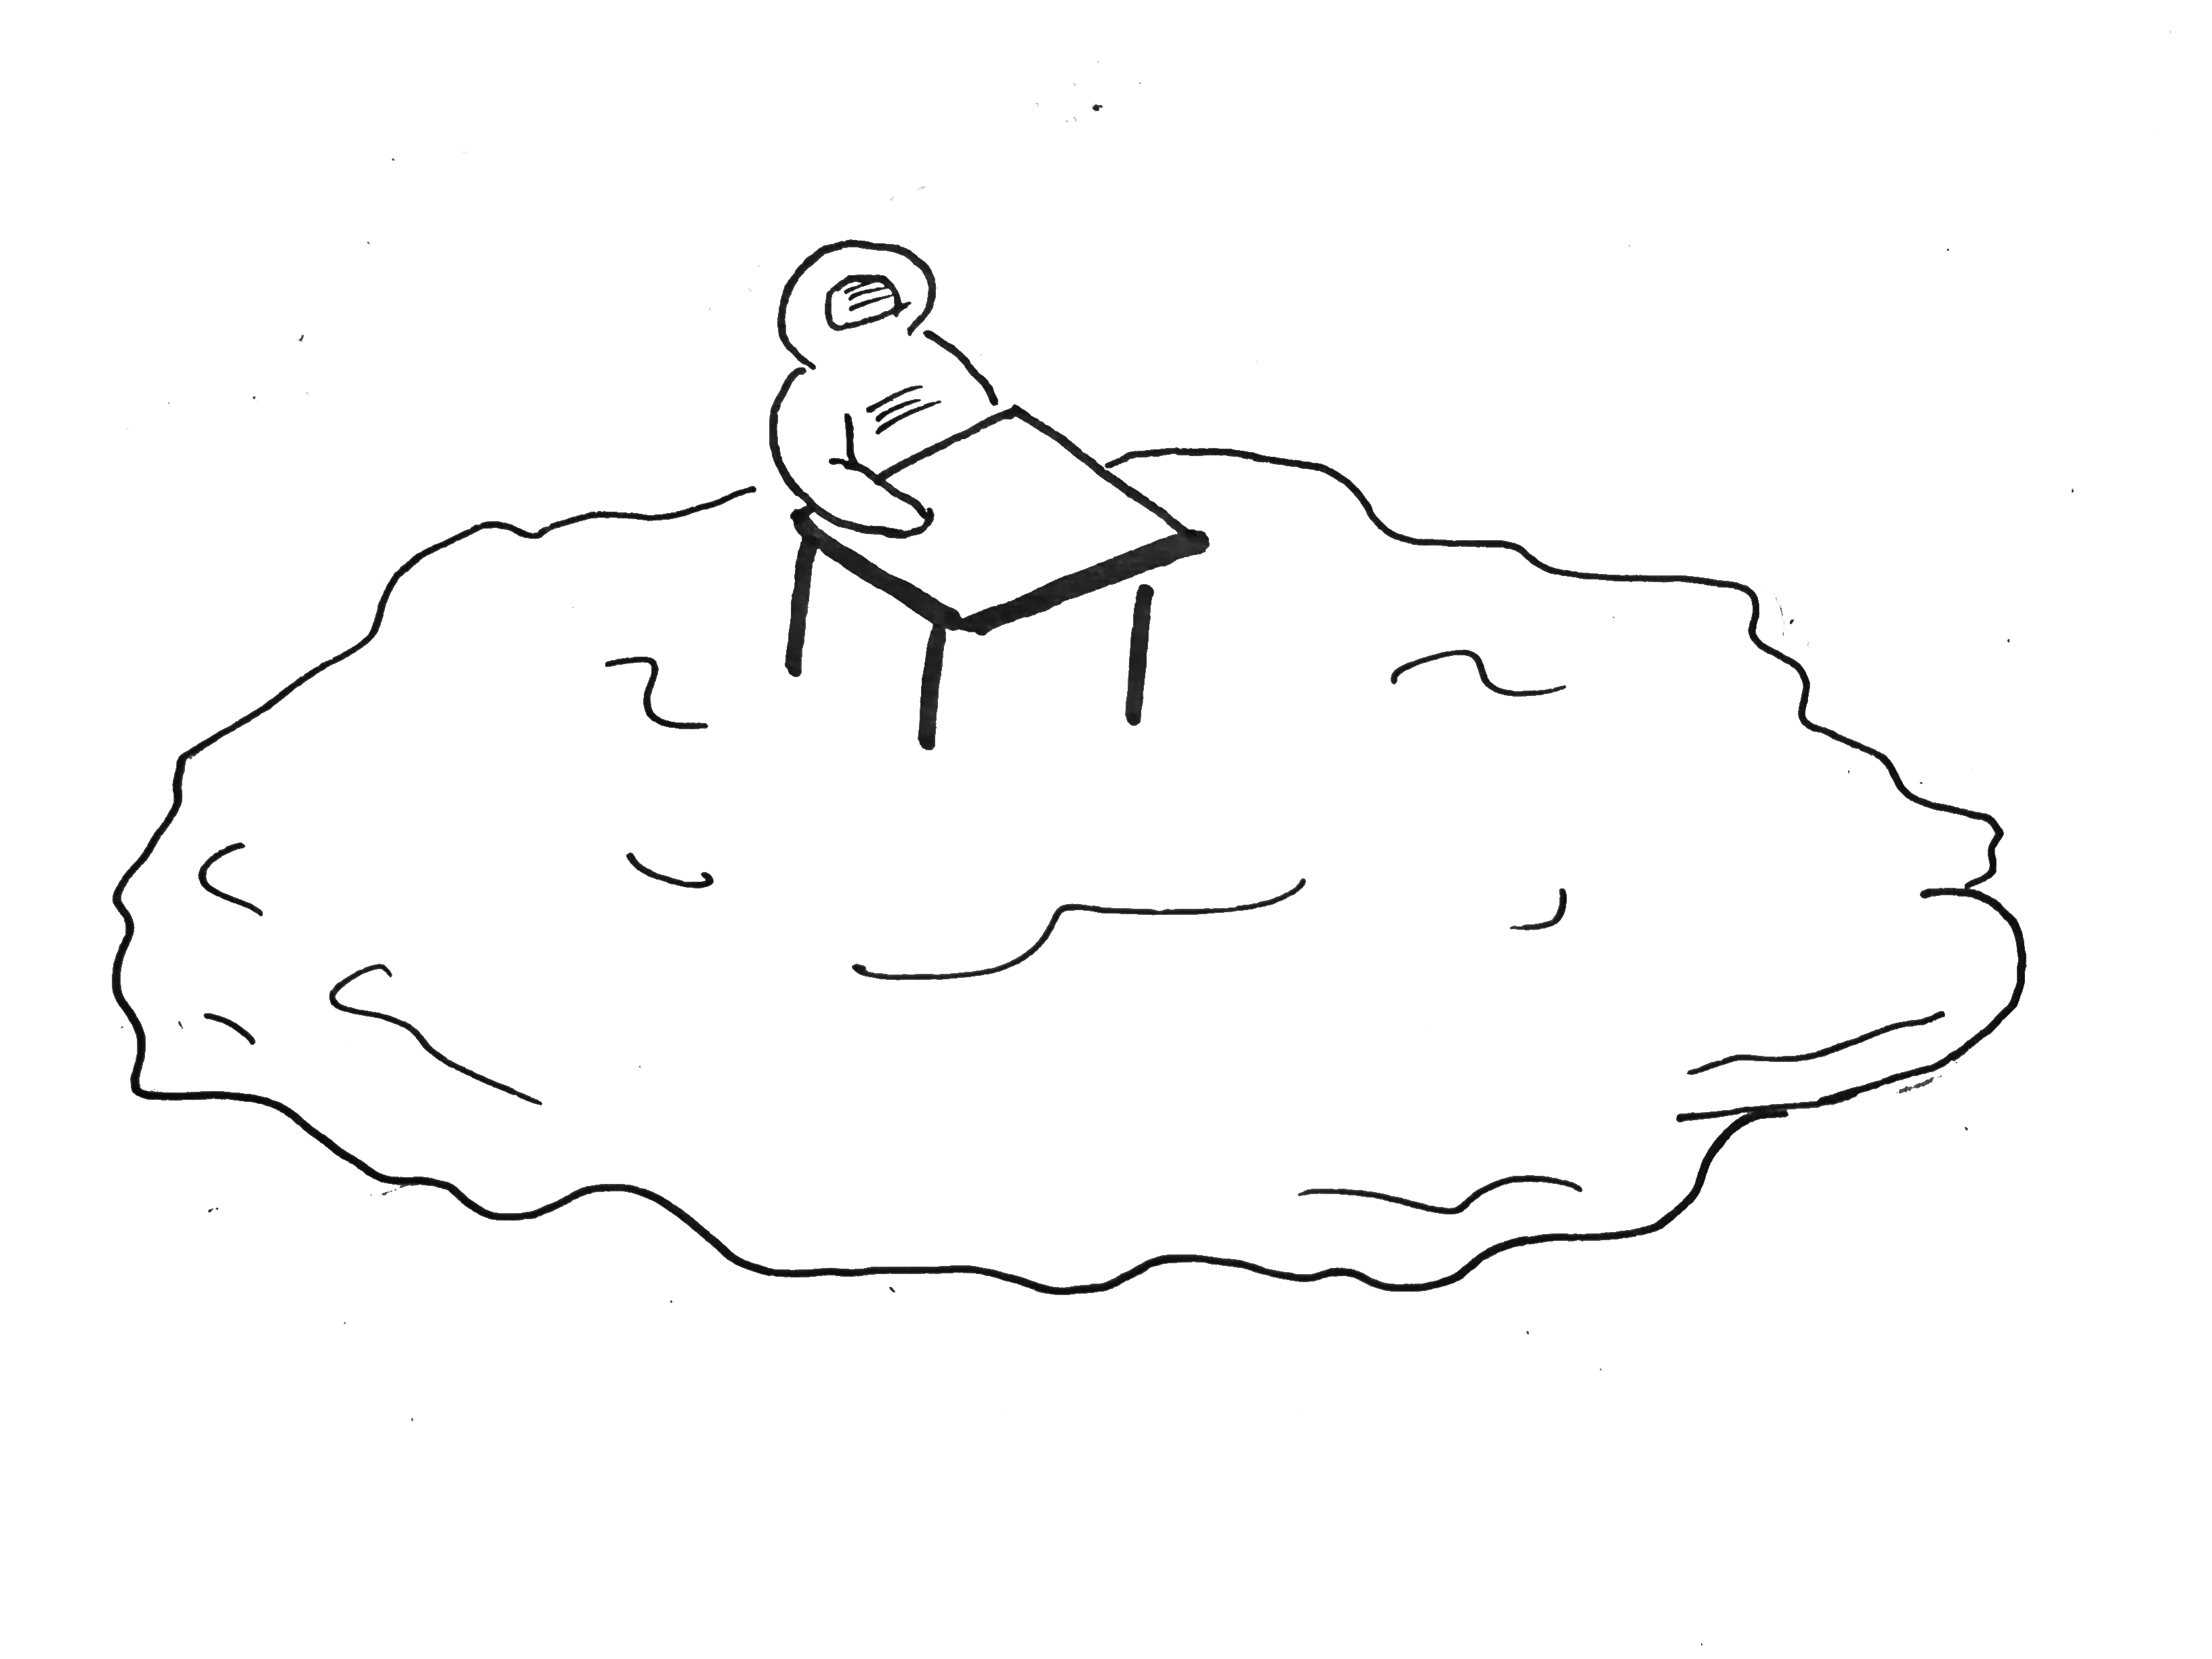
\includegraphics[width=14cm]{img-archaeopteryx/qfwfq_asteroide}};
			\draw [black,ultra thick] (6,6.5) rectangle (24,-6.7);
		\end{scope}
		%
		\begin{scope}[shift={(0,-28)}]
			\node at (22,0) {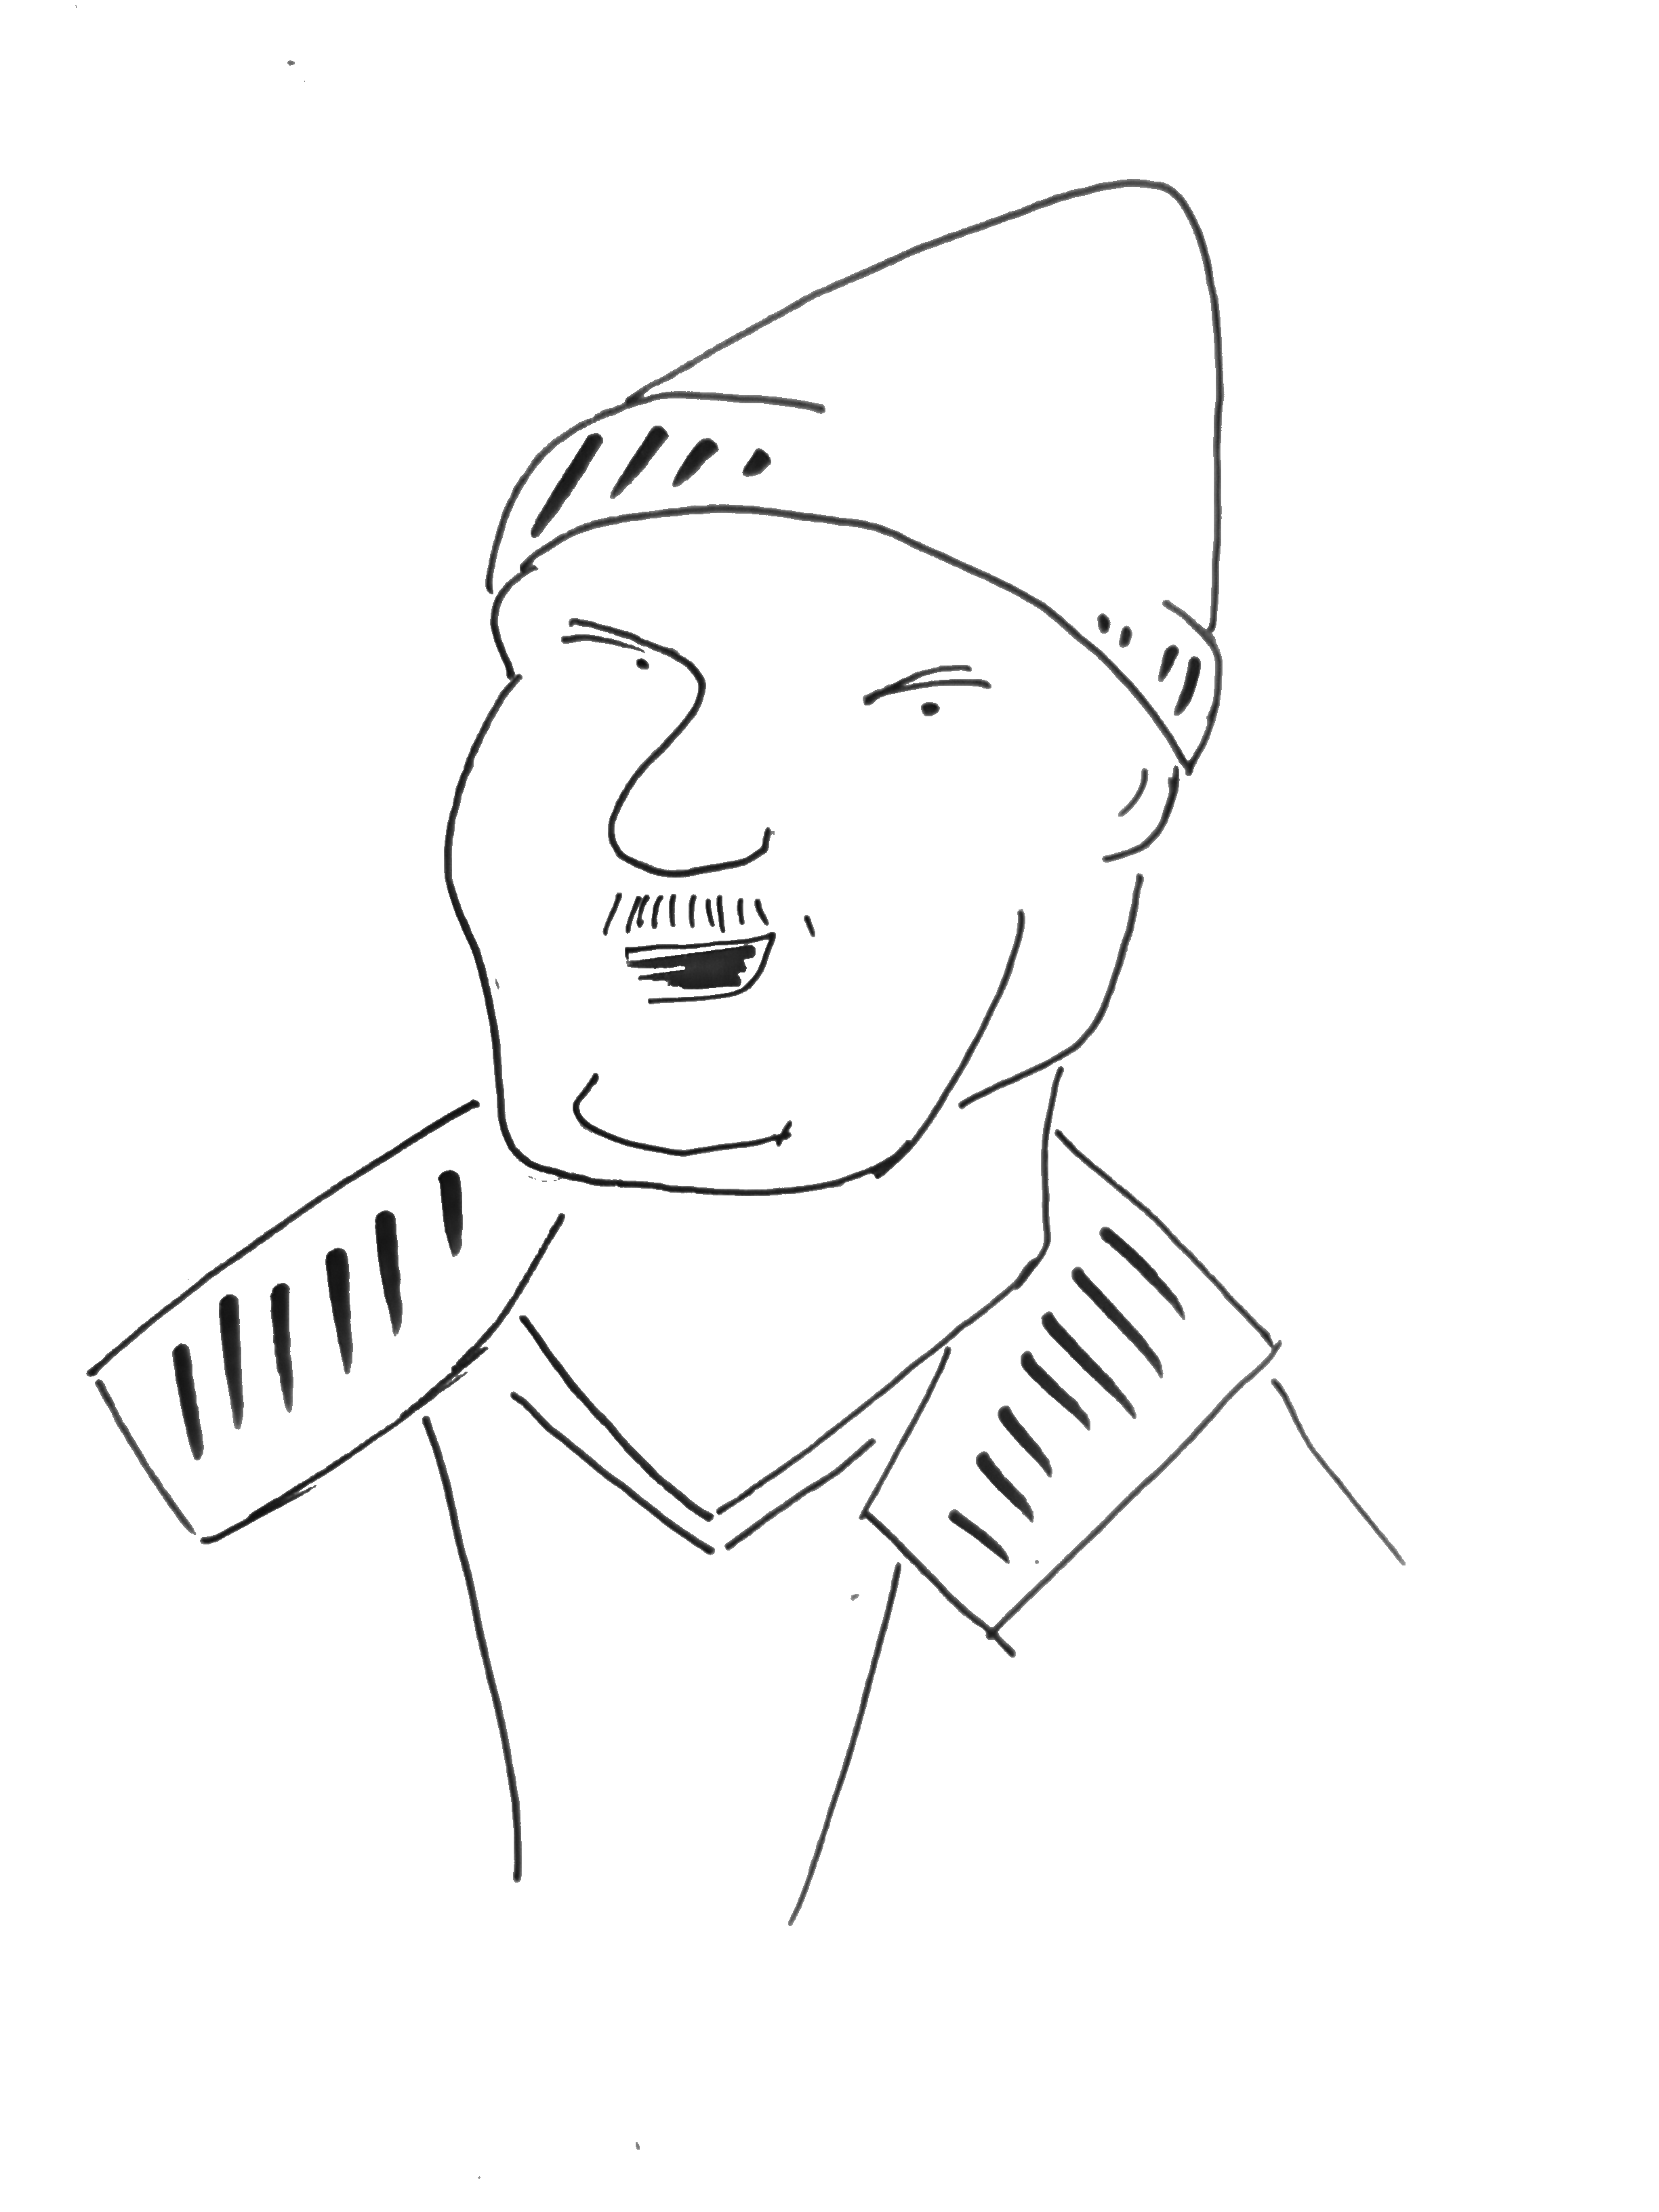
\includegraphics[width=12cm]{img-archaeopteryx/eric_walter_elst}};
			\node (example-textwidth-2) [right, align=left, text width=15cm, color=black, font=\fontsize{18pt}{19pt}\selectfont] at (2,0) {Ci furono diverse resistenze da parte degli astronomi, ma alla fine il buon Eric capi' la mia esigenza: ricordare un caro amico dei tempi d'oro di quando il pianeta era un posto invivibile per i mammiferi. E cosi' questo sasso spaziale posto a 3 unita' astronomiche dalla Terra prese il nome di 9860 Archaeopteryx.\\E' stato un caro compagno di pigolate e un sincero amico: si andava a caccia di prede un po' a terra un po' in aria. D'altra parte all'epoca non sapevamo nemmeno se eravamo dinosauri o uccelli. E aveva anche poca importanza.\\Se e' per questo neanche gli scienziati si sono ancora messi d'accordo su cosa era il caro Archaeo. E la cosa non mi stupisce: mica c'erano, loro!};
			\draw [black,fill=white,ultra thick] (18.8,-5.5) rectangle (23.5,-6.5);
			\node (example-textwidth-2) [right, align=left, text width=5cm, color=black, font=\fontsize{14pt}{15pt}\selectfont] at (19,-6) {Eric Walter Elst};
		\end{scope}
		%
		\begin{scope}[shift={(0,-32)}]
			\node at (15,-12) {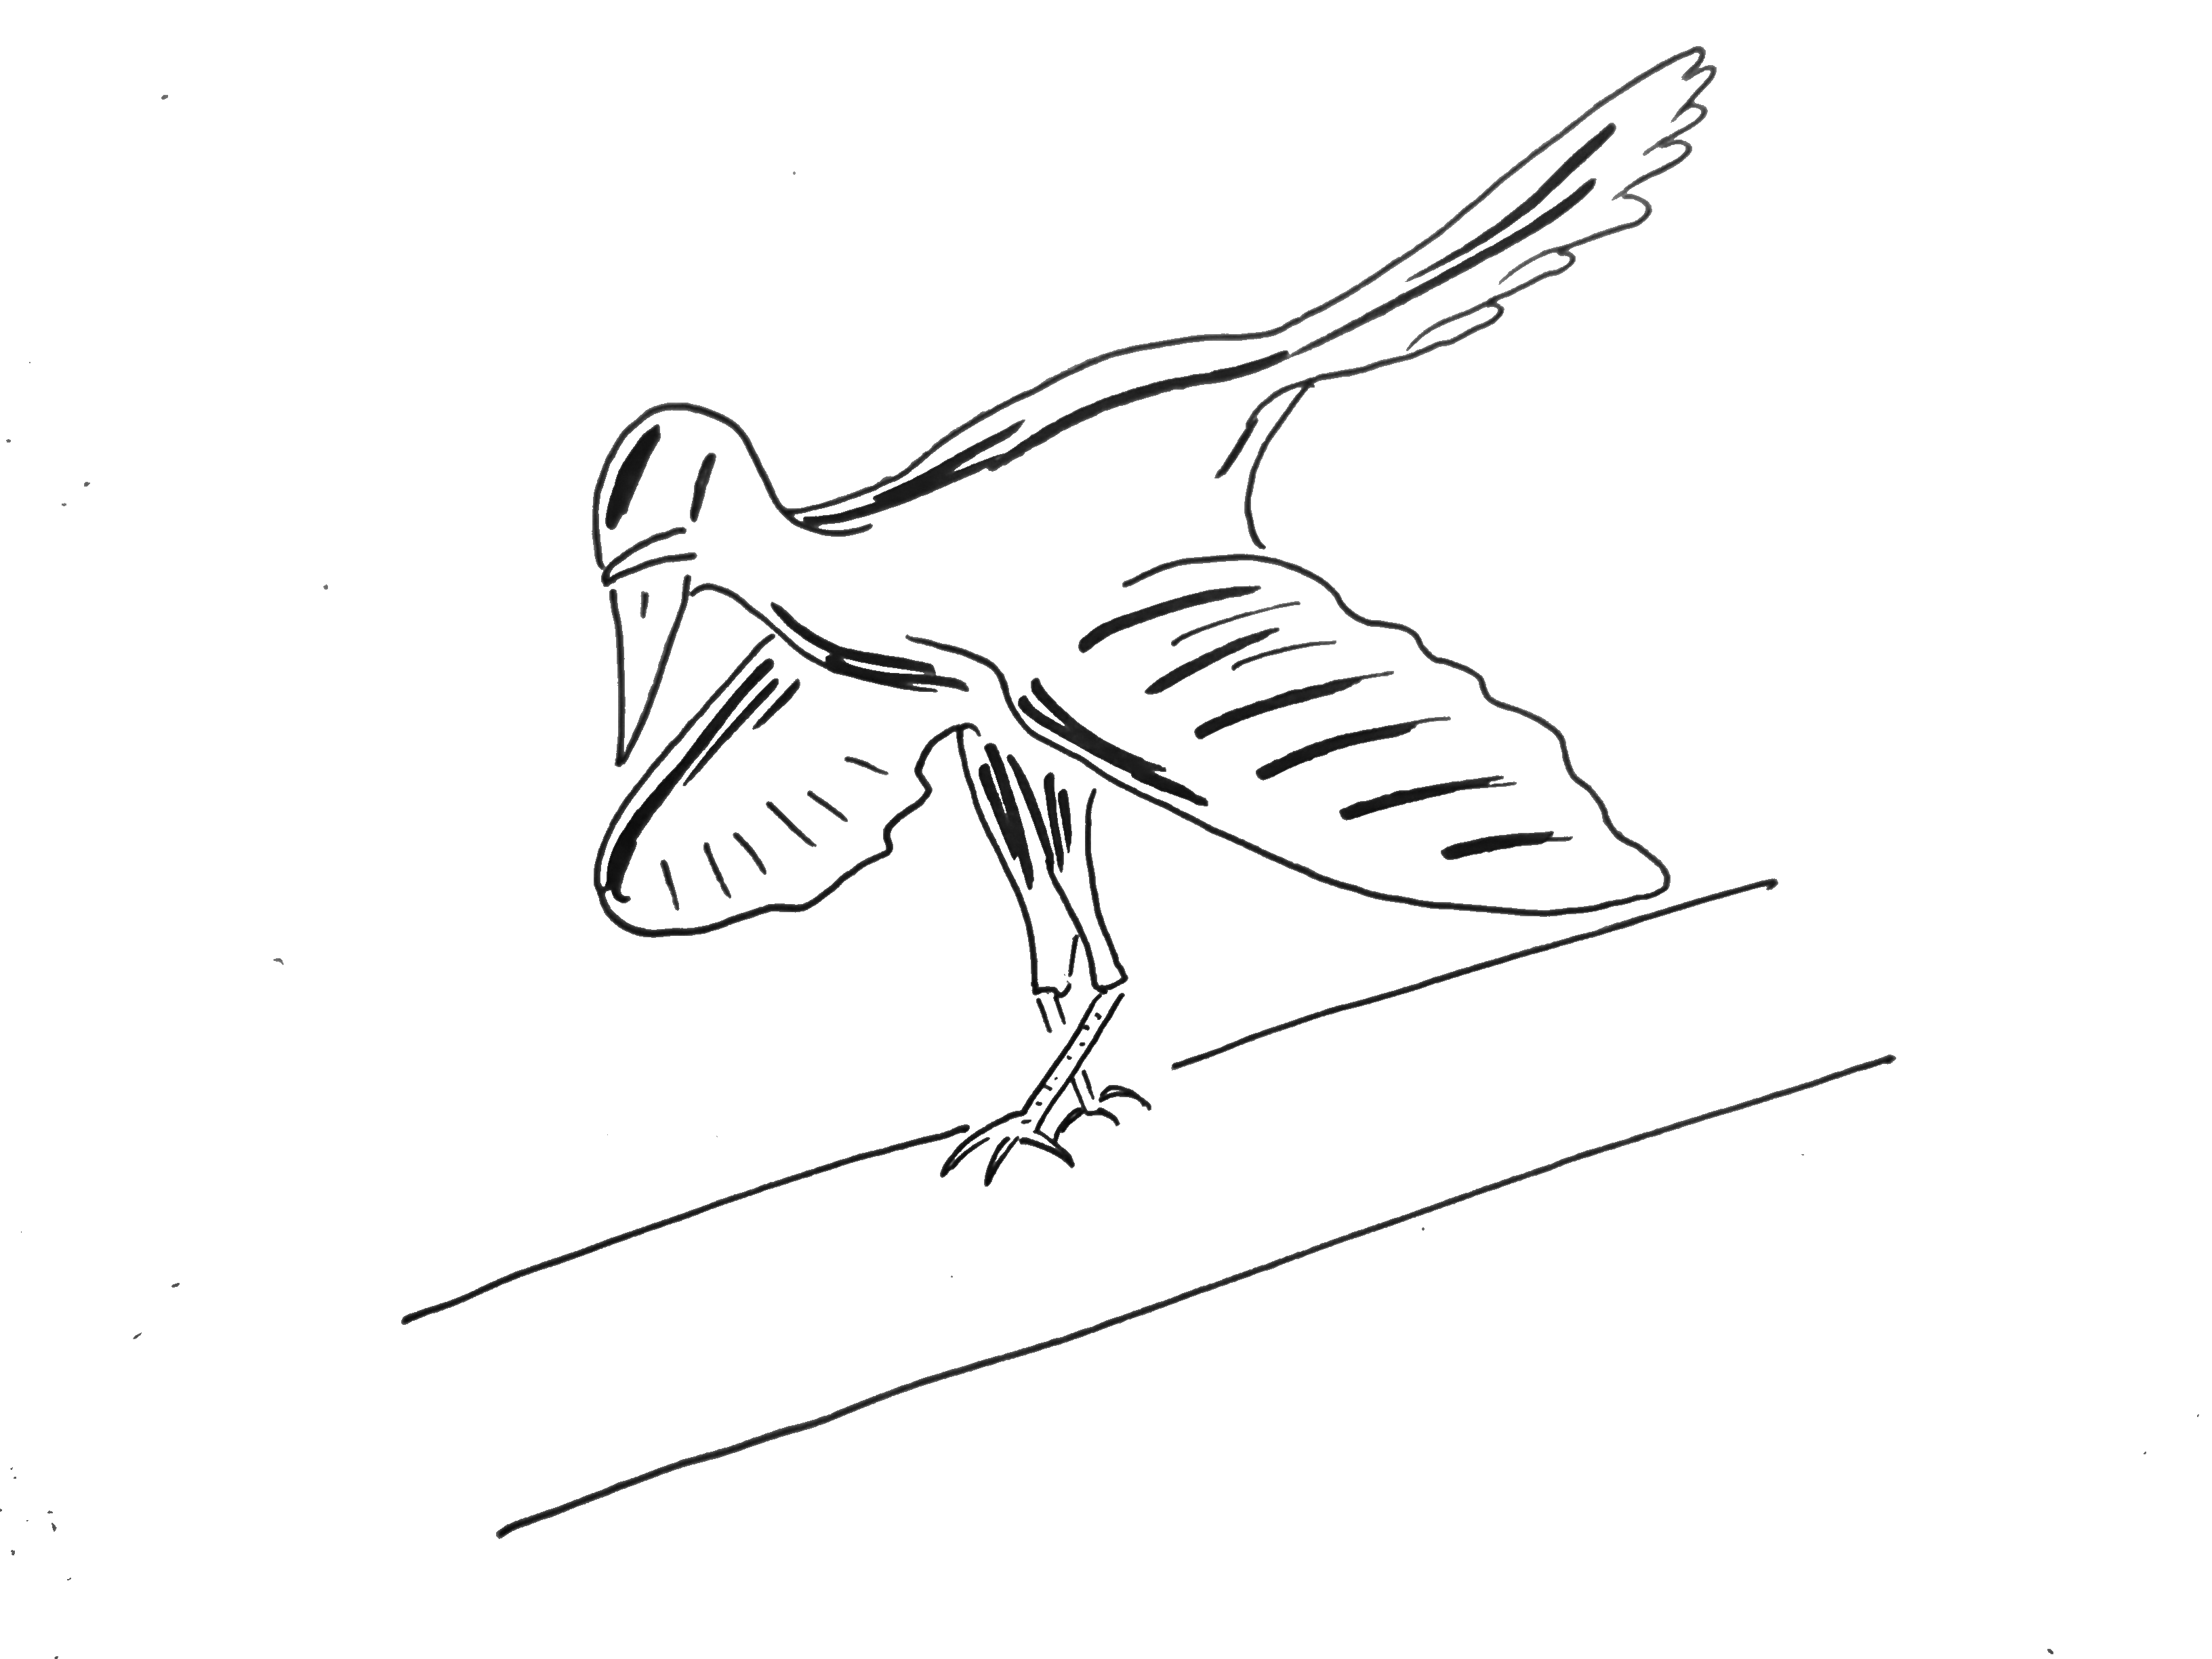
\includegraphics[width=25cm]{img-archaeopteryx/archaeopteryx}};
		\end{scope}
		%
		\begin{scope}[shift={(0,-55)}]
			\node at (7,-2) {
\includegraphics[width=5cm]{img-archaeopteryx/piuma}};
			\node (example-textwidth-2) [right, align=left, text width=12cm, color=black, font=\fontsize{18pt}{19pt}\selectfont] at (12,-2) {Il mio buon amico, ormai estinto da 150 milioni di anni o giu' di li', ha lasciato poche tracce dietro di se: appena 12 fossili, inclusa una piuma. Pero' ricordo ancora il suo canto meraviglioso:};
			\node (example-textwidth-2) [right, align=left, text width=12cm, color=black, font=\fontsize{18pt}{19pt}\selectfont] at (12,-5) {"Koaxpf... Koaxpf... Koaaaccch..."};
			\node (example-textwidth-2) [right, align=left, text width=12cm, color=black, font=\fontsize{18pt}{19pt}\selectfont] at (12,-7) {Era portato per il canto! Non trovate anche voi?};
		\end{scope}
		%
		\begin{scope}[shift={(0,-66)}]
			\node at (27,0) () {
\includegraphics[width=3.7cm]{licenza}};
			\node at (15.5,-0.1) {\textcolor{black}{\fontsize{14}{15}\selectfont Testo e illustrazioni, esclusa la piuma: @ulaulaman - Gianluigi Filippelli}};
		\end{scope}
	\end{tikzpicture}
%
\end{document}
